 \documentclass[11pt, oneside, letterpaper]{article}
\usepackage{graphicx}
\usepackage{enumerate}
\usepackage{amsmath}
\usepackage{amssymb}
\usepackage[cm]{fullpage}
\RequirePackage[T1]{fontenc}
\RequirePackage{times}
\RequirePackage{charter} % Default font
\newcommand{\tasksep}{\noindent\underline{\hspace{\textwidth}}}

\usepackage{color}
\newcommand{\mf}[1]{{\bf\textcolor[rgb]{1.00,0.00,0.00}{MF: #1}}}

\begin{document}

\title{\huge\textbf{Planning Algorithms in AI \\  PS2: Sampling-based Planning}}
\author{Gonzalo Ferrer\\Skoltech}
\date{\today}
\maketitle

This problem set has two tasks  and is individual work. You are encouraged to talk at the conceptual level with other students, discuss on the equations and even on results, but you may not show/share/copy any non-trivial code.


\section*{Submission Instructions}
Your assignment must be submitted by 11:59pm on {\bf November 29}. You are to upload your assignment directly to Canvas as {\bf two} attachments:

\begin{enumerate}
\item A \texttt{.tar.gz} or \texttt{.zip} file \textit{containing a directory} named after your uniquename with the structure shown below.

\texttt{yourname\_ps2.zip}:\\
\texttt{yourname\_ps2/all\_provided\_code\_file.py}\\
\texttt{yourname\_ps2/data.pickle}\\
\texttt{yourname\_ps2/any\_your\_code\_file.py (or .ipynb)}\\
\texttt{yourname\_ps2/solve\_4R.mp4 (or .gif)}\\


\item A PDF with the written portion of your write-up. Scanned versions of hand-written documents, converted to PDFs, are perfectly acceptable (reduced size).  No other formats (e.g., .doc) are  acceptable.  Your PDF file should adhere to the following naming convention: \texttt{yourname\_ps2.pdf}.

\end{enumerate}

Homework received after 11:59pm is considered late and will be penalized as per the course policy. The ultimate timestamp authority is the one assigned to your upload by Canvas.  No exceptions to this policy will be made.

\textbf{Please} make sure all your code is \textit{well structured, understandable and reproducible}!


\section*{Task 1: Visualization (20 points)}


The Workspace is a continuous 2D area: $\mathcal{W} = \mathbb{R}\times\mathbb{R}$ with \textit{six obstacles}. Here, we work with the 2D manipulator mechanism which consists of 4 links, "root" joint is placed in (0, 0). The configuration can be expressed as $\bold{q} = [\theta_1, \theta_2, \theta_3, \theta_4]$, where $\theta_i \in (-180; 180]$ is the angle of the link relative to manipulator's joint in degrees. 

\begin{itemize}
    \item Both angles and coordinates on the plane are continuous variables.
    \item Note that intersection of the links is allowed (imagine that all links are in different planes).
\end{itemize}

\begin{figure}
    \centering
    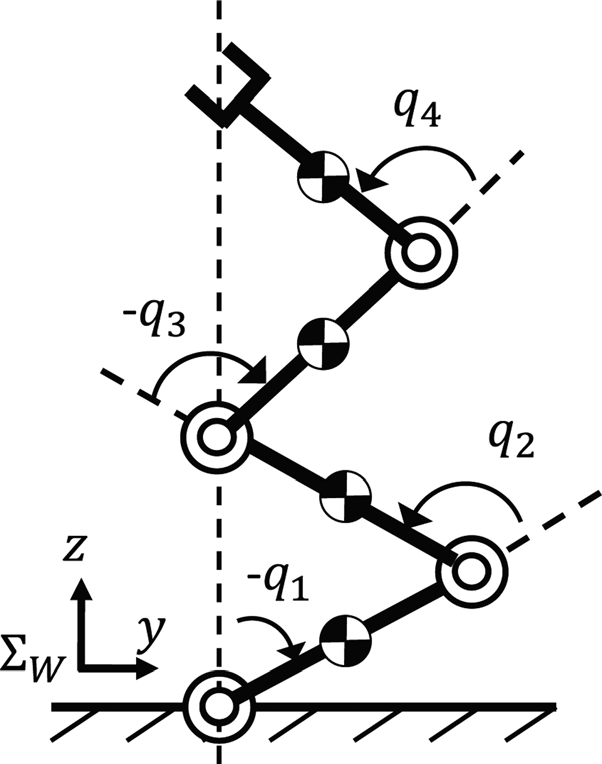
\includegraphics[width=0.25\columnwidth]{Figures/Four-link-manipulator-Fig-4-Configuration-of-manipulator.png}
    \caption{The example of the 4R four-link manipulator.}
    \label{fig:Four-link-manipulator-Fig-4-Configuration-of-manipulator}
\end{figure}



All the required data can be obtained from \texttt{data.pickle}. See \texttt{main.py} to check how to load the data. The pickle file consist of the dictionary with the following fields:
\begin{itemize}
\item \texttt{start\_state} and \texttt{goal\_state} are the \texttt{[4,]} arrays with the starting configuration $\mathbf{q}_{start}$ and the target configuration to reach $\mathbf{q}_{goal}$.
    \item \texttt{obstacles} is the \texttt{[6, 3]} array of the circular obstacles in format $[x_i, y_i, R_i]$, where $R$ -- radius and $i = 1, \dots, 6$.
    \item \texttt{collision\_threshold} is the float number that defines minimal allowed distance to the obstacle
\end{itemize}

To see how display the manipulator in desired state, check \texttt{environment.py} file.


\begin{enumerate}[A.]

\item (10 pts)
Visualize the manipulator in the start state and target state. Comment on your thoughts about comparison the discretized orientation space from PS1 vs continuous orientation space in current problem set.

\item (10 pts)
Visualize the manipulator in 4 random orientations that include both colliding and non-colliding configurations. Check what does the \texttt{ManipulatorEnv.check\_collision} function returns for those configurations. Comment on your observations.


\end{enumerate}

\section*{Task 2: Rapidly-exploring Random Trees (RRT) (80 points)}
For this task, you will implement the RRT algorithm to solve the path planning for the 4R manipulator. Follow the material explained in class 

\begin{enumerate}[A.]

\item (10 pts) Implement a collision check between any two configurations. To do that, generate a random configuration $q$ and a small increment over it, for arbitrary size.
In order to implement the collision between two configurations, you have to check a sequence of configurations connecting them, in the limit representing a connectivity path as discussed in Lecture 3. Choose a sequence of some size and comment your choice.
To do that, you may want to use function \texttt{angle\_linspace} from \texttt{angle\_utils.py}.

Also, the simple configuration check is implemented in the function \texttt{ManipulatorEnv.check\_collision}, in order to check if the the manipulator is in collision at any point towards the new configuration.

Show in the same visualization the sequence of manipulator configurations for a negative collision check. Show a second figure with a positive collision check, starting from a valid initial configuration and ending in a valid configuration but colliding on its intermediate configurations.


\item (40 pts)
You need to implement the RRT algorithm for agent in continuous domain.
The starting configuration of the agent is \texttt{(0, 0, 0, 0)} and the goal configuration is \texttt{(-180.0, -60.0, 72.0, -60.0)}.
For searching nearest pose use $L_1$ \texttt{distance} between two configuration vectors:
\begin{equation}
    distance = \| \bold{q_2} - \bold{q_1} \|_1
\end{equation}

As a maximum allowed rotation for each joint we suggest you to use $10$ degrees.
You may want to use function \texttt{angle\_difference} from \texttt{angle\_utils.py} and the two-configuration collision check developed above.

Save the result of calculated plan in \texttt{solve\_4R.mp4} (or other video extension) using provided \texttt{animate\_plan} function from \texttt{video\_util.py}. If you want to add more smoothness to the video, you can add additional intermediate configurations, but it's optional.


\item (10 pts)
Comment on how many states have been visited? What is the final trajectory size? Can you comment on the optimality of the plan? You can also collect some observations and statistics across multiple runs.

\item (10 pts)
Try to change weight of rotation in calculation of distance between two agent positions. We suggest you to build a distance function based on weighted sum of the angle distances.
% and also a distance function based on joint positions.
Comment on the results.
\item (10 pts)
Try to change step size used for RRT branches. Comment on the results.
\end{enumerate}
\end{document}
